%%=============================================
% !Mode:: "TeX:UTF-8"
% !TEX program  = XeLaTeX
%%=============================================
% 模板名称:HITSZThesis
% 模板版本:V2.2
% 模板作者:杨敬轩(Jingxuan Yang)
% 联系作者:yangjingxuan@stu.hit.edu.cn & yanglatex2e@gmail.com
% 模板交流:QQ群:1039392552,加群请备注LaTeX、HITSZThesis相关说明
% 模板适用:哈尔滨工业大学(深圳)本科毕业设计(论文)
% 模板编译:XeLaTeX,编译两次,两次,两次!!!
%          GNU make 工具:make thesis
%          compile.bat 批处理脚本:compile.bat thesis
%          更多编译细节详见说明文档:hitszthesis.pdf
% 更新时间:2020/03/05
% 模板帮助:请**务必务必务必**阅读 hitszthesis.pdf 说明文档,文档查看方法:
%          cmd 命令行:texdoc hitszthesis
%          推荐前往模板的GitHub仓库获取最新文件,地址:
%          https://github.com/YangLaTeX/hitszthesis
%%=============================================

% 设置文档类别为<hitszthesis>
\documentclass{hitszthesis}

% 模板提供以下选项
% 1. 封面标题单行或多行显示:
%%  onerow(默认,单行),tworow(两行)
% 2. 封面第二页下划线内容居中或居左显示:
%%  infocenter(默认,居中),infoleft(居左)
% 3. 正文数学字体选项:
%%  newtxmath(默认,凑合),mtpro2(非常推荐)
%%  将 newtxmath 设置为默认数学字体仅为了避免同学未安装mtpro2字体
%%  会产生的编译错误
%%  !mtpro2为非免费字体,CTAN禁止提供下载链接,需自行下载该字体

% 示例:两行,居左,mtpro2字体,将<\documentclass{hitszthesis}>注释,
% 且将下面语句取消注释
%\documentclass[tworow, infoleft, mtpro2]{hitszthesis}

% 自定义设置与额外加载的宏包请写在 \file{hitszthesis.sty} 里
% 预设该文件为空
\usepackage{hitszthesis}

% 填写封面信息
% !TEX root = ../main.tex

%TC:ignore

% 论文标题
\thesistitle{基于神经网络的机器人智能抓取研究}
% 标题拆分为两行
% 第一行标题
\titleone{基于神经网络的}
% 第二行标题
\titletwo{机器人智能抓取研究}
% 学校名称
\schoolname{哈尔滨工业大学(深圳)}
% 学院名称
\departname{机电工程与自动化学院}
% 专业
\majorin{机械设计制造及其自动化}
% 姓名
\authorname{杨敬轩}
% 学号
\studentID{SZ160310217}
% 答辩日期
\dateinput{2020年6月7日}
% 指导教师
\instructor{XX 教授}

%TC:endignore

%%=============================================
% 开始写文章
% !!注意本文仅作为排版格式示例,并不作为毕业论文规范
\begin{document}

% 若题目过长,则需使用以下命令调整封面第二页下划线长度
%\infowidth = 8cm

% 生成封面两页
\maketitle

% 开始写前言部分
\frontmatter

% 中文摘要
% !TEX root = ../main.tex

% 开始写摘要
\begin{abstract}
 
近年来,基于神经网络方法的机器人智能抓取物体的研究方兴未艾。本文首先介绍了该研究的背景,采用神经网络的方法进行机器人智能抓取研究是一个可行的方案。

而后,本文总结归纳了神经网络在机器人智能抓取领域的研究历史与研究现状。由实值神经网络的三个里程碑意义的模型到复值神经网络的兴起,神经网络的模型得到了极大地扩展。基于深度学习的方法已经在机器人视觉识别领域取得了重大的成就,识别要抓取的物体图像以后,机器人的抓取策略也很有讲究。

本文还重点介绍了基于三种不同的神经网络方法进行的机器人智能抓取研究。首先是基于复值神经网络的方法,该方法包含离散、连续、多值三种模型,复值神经网络以其自然的复数处理能力,使得图像等常需频域处理的信号有了直接的表达和处理方式。

然后是基于轻量级卷积神经网络的方法,目前基于神经网络的机器人抓取位姿预测方法的研究使用的网络结构通常具有大量的参数,需要大量的计算和存储资源。基于 SqueezeNet 的轻量级卷积神经网络抓取预测模型在不降低准确率的情况下,网络模型更小,需要的存储资源更少,速度更快。

最后是基于级联卷积神经网络的方法,该方法提出一种抓取姿态细估计的卷积神经网络模型 Angle-Net,在此基础上,提出一种两阶段级联式抓取位姿检测模型。

% 中文关键词
\keywords{轻量级;卷积神经网络;复值神经网络;级联神经网络;轻量级卷积神经网络;位姿检测模型}
\end{abstract}

% 英文摘要
% !TEX root = ../main.tex

% 英文摘要
\begin{abstracten}

In recent years, the research of intelligent object grabbing by robots based on neural network method is in the ascendant. Firstly, this paper introduces the background of this research, and it is a feasible scheme to apply the neural network method to the intelligent grasping of robots. 

Then, this paper summarizes the research history and status quo of neural network in the field of robotic intelligent grasping. From the three milestone models of real-valued neural networks to the emergence of complex-valued neural networks, the model of neural networks has been greatly expanded. The method based on deep learning has made great achievements in the field of robot vision recognition. After recognizing the object image to be grasped, the strategy of robot grasping is also very exquisite. 

This paper also focuses on the intelligent grasping of robots based on three different neural network methods. Firstly, the method based on complex-valued neural network includes three models: discrete, continuous and multi-valued. Complex-valued neural network, with its natural complex processing ability, makes the signal which often needs to be processed in frequency domain, such as image, have a direct expression and processing mode. 

Then it is based on the method of lightweight convolution neural network. At present, the network structure used in the research of robot grasping pose prediction method based on neural network usually has a large number of parameters, which requires a lot of computing and storage resources. The grabbing prediction model of lightweight convolutional neural network based on SqueezeNet has smaller network model, less storage resources and faster speed without reducing accuracy. 

Finally, based on the method of cascade convolution neural network, a convolution neural network model Angle-Net for fine grabbing attitude estimation is proposed. On this basis, a two-stage cascade grabbing pose detection model is proposed.

% 英文关键词
\keywordsen{Lightweight, Convolutional Neural Network, Complex Neural Network, Two stage cascade grabbing pose detection model}
\end{abstracten}

% 生成目录
\tableofcontents

% 开始写正文
\mainmatter

% 第1章
% !TEX root = ../main.tex

% 第1章的标题
\chapter{绪论}

% 正文内容,注意LaTeX分段有两种方法,直接空一行或者使用<\par>
% 默认首行缩进,不需要在代码编辑区手动敲空格
随着社会发展,人口老龄化,劳动力短缺等问题逐渐凸显,对服务机器人的需求也越来越大,但是服务机器人所工作的非结构化环境也带来了许多技术难题,其中十分主要的一个问题就是非结构环境中机器人的自动抓取,因为抓取是机器人与现实世界交互的主要方式之一。不同于工业机器人在结构化环境中对工件的抓取,服务机器人在非结构化环境下的自动抓取面临着诸多挑战,例如动态化环境、光照变化、物体间存在相互遮挡,以及最主要的,非结构化环境中除了已知的物体,还有大量未知物体。对于非结构化环境中工作的服务机器人,预先获取所有需要进行抓取的物体的模型是不现实的,因此机器人必须能够对未知的物体在线进行快速稳定可靠的抓取规划。

为了解决上述问题,常用的一种做法就是使用机器学习方法来学习从传感器数据提取出的特征表达到抓取位姿的映射关系,相比于建立物体的模型库来保存抓取经验,机器学习方法可以在没见过的物体上进行抓取经验的迁移。在这个领域中,一些传统的方法通常借助于人工设计的特征来表示和存储抓取经验,并训练分类器,但人工设计的特征往往只针对于某一种特定物体或任务有效,且人工设计特征的工作量大难度高,很难在其他场景进行使用。
 
近年来,以卷积神经网络(Convolutional Neural Network, CNN)为代表的深度学习技术,在计算机视觉和机械设备健康监测等诸多领域取得了重大的突破,在一些领域中达到了超过人类的性能。卷积神经网络可以通过大量数据的训练挖掘出适合于当前任务的特征表达,由于通常卷积神经网络需要堆叠很多层来提高特征表达能力,因此参数较多,需要使用比传统机器学习算法更多的标注数据来进行训练,抑制过拟合提高算法的泛化能力。

在机器人抓取规划领域,使用卷积神经网络学习的特征取代人工设计的特征来对抓取进行表示和分类有很大的优势和应用前景。首先,相比于人工设计的特征,卷积神经网络通过大量数据的学习可以挖掘出泛化能力更强效果更好的特征,可以进一步提高抓取规划算法的性能,且省去了复杂的人工特征设计工作。其次,随着硬件计算力和仿真软件性能的提升,视觉传感器的普及,目前已有许多通过实验或者仿真收集的机器人抓取数据集可供使用。
 
综上,有了足够的数据以及合理设计的卷积神经网络结构就可以建立更高性能的自动抓取规划算法,进而提高服务机器人在非结构化环境的交互能力,提高其自主化和智能化程度,提高服务机器人的实用性和推进产业落地。因此,基于卷积神经网络的机器人自动抓取规划具有重要的研究价值,可以带来巨大的经济效益。

% 第2章
% !TEX root = ../main.tex

% 第2章的标题
\chapter{文献综述}

% 第2章第1节的标题
\section{实值神经网络发展历程}

% <\upcite{}>为在右上角引用参考文献命令
% <\cite{}>为在正文中引用参考文献命令
% 目前不支持[1-6]类型的引用,需手动填写<$^{[1\text{-}6]}$>

人类利用人工神经网络对生物神经网络的结构、机理和功能模拟的研究,经历了近半
个多世纪漫长而又曲折的过程。具有里程碑意义的是如下三个模型\upcite{bibc1,bibc2}。

1943年神经生理学家McCulloch和数学家Pitts提出的第一个人工神经网络模型:
McCulloch-Pitts模型\upcite{bibc3},成为神经网络研究的开端。1949年心理学家D.O.Hebb在文献\upcite{bibc4}中提出了神经元之间突触联系强度可以改变的假设,并据此提出了神经元学习的准则,为神经网络的学习算法奠定了基础。这些重大进展促进了神经网络早期的研究。

1958年Rosenblat将McCulloch和Pitts的工作与Hebb的工作结合在一起,设计出的
一种称为感知机的神经网络模型\upcite{bibc5},首次把人工神经网络的研究从理论付诸工程实践,引起了许多科学家的兴趣。不过在1969年,人工智能创始人之一Minsky和Papert出版了以《感知机》为名的书\upcite{bibc6},书中从数学上深入分析了感知机的原理,指出了其局限性并从理论上对感知机的原理给予了沉重的打击,使得神经网络早期的研究热潮迅速降温,并开始陷入低潮和休眠状态。

% <\/>命令解决fi、ff等上边连接在一起的问题
1982年和1984年美国加州理工大学的生物物理学家J.J.Hopf\/ield提出了Hopf\/ield神经网络\upcite{bibc7,bibc8}。Hopf\/ield神经网络模型的提出具有划时代的伟大意义,使得神经网络的研究从体眠的状态开始复苏。Hopf\/ield在文献\cite{bibc7,bibc8}中设计出用电子电路实现这一网络的方案,从而为神经计算机的研究奠定了基础。更为重要的是他把设计出的神经网络应用于联想记忆以及解决优化领域一直困扰的TSP问题,并取得了巨大的成功,这些重大进展大大促进了神经网络的研究。此外,他还通过引入类似于Lapunov函的“计算能量函数”的概念对网络的动力学特性进行了分析并给出了网络稳定性的条件,从而开启了神经网络稳定性研究。

% 节标题
\section{复值神经网络的兴起}

复值神经网络(Complex-valued Neural Network)是实值神经网络在复数域的推广。相比实值神经网络,复值神经网络的起步稍晚。其历史可追溯到1975年Widrow提出的复值最小均方(LMS)算法,该算法后来被广泛运用于信号处理领域\upcite{bibc9}。但正如复数的出现和被人认可经历了一个漫长的过程一样,复值神经网络在出现后的相当长时间,并未引起人们的重视。直至近几年来,随着神经网络应用领域的不断扩展,许多需要处理复数信号的领域也提出了用神经网络解决其相关问题的要求,例如量子力学、电磁学、光电子、图像、遥感、时间序列分析等。在这些领域中,基于复数信号的表示、分析和处理具有极大的便利,而复值神经网络则能直接处理复数信号,因而很自然地使二者联系在一起。事实上,在需要幅值和相位(或理解为大小和方向)两方面信息来表示同一信号的场合,运用复值神经网络较之实值神经网络,要更为直接。尽管可以用2个实值神经网络分别表达此类信号的大小和方向(或实部和虚部),但正如复数虽然只是两个实数按某种规则而连接,但依然有其独立于实数而存在的必要性一样,复值神经网络由于复数有实部和虚部,且复数运算规则的特殊性等原因,在其实现和运用过程中表现出一些实值神经网络所不具有特质,因此复值神经网络也不能简单地理解为可用2个实值神经网络所取代。而且在将神经网络从实数域到复数域的推广中,并不是像表面上理解的那样:仅是简单地将一个变量从实数变成复数。如果这样做的话,许多诸如奇异等意想不到的问题就有可能发生\upcite{bibc10}。

作为复值神经网络研究领域的先导者,日本的Akira Hirose教授总结了近年来复值神经网络的研究成果,并出版一本名为《复值神经网络的理论及应用》专著\upcite{bibc10}。书中总结了近年来复值神经网络理论的发展和应用情况。

% 节标题
\section{抓取物体图像识别}

近年来,基于深度学习的方法已经在包括视觉识别\upcite{bib1,bib2},语音识别和自然语言处理等任务上取得了重大成就。美国康奈尔大学 Lenz 等\upcite{bib3}借鉴深度学习在图像检测及图像识别等任务中的成功经验,提出了基于深度学习的机器人抓取检测的方法\upcite{bib3,bib4}。与传统的依靠人工经验抽取样本点特征的方式相比,基于深度学习的机器人抓取检测的方法可以自动学习如何识别和提取待抓取位置的特定特征。越来越多的机器人学者研究如何将深度学习的方法应用于机器人抓取检测上从而使机器人具备更强大的智能。大部分研究学者都是将深度学习的方法用来学习不同形状和位姿的物体的末端执行器的最佳配置,基于深度学习的深层表达能力学习的参数为每个图像预测多个抓取位置进行排序来找到最佳抓取位置。

基于深度学习的方法,Lenz 等\upcite{bib3}提出了基于稀疏自编码器的两步级联抓取检测系统,构建两个大小网络用于提取 RGB-D 输入数据的抓取特征,采用滑动窗的方法搜索抓取框,最后在网络顶层添加支持向量机(Support Vector Machine,SVM)作为分类器的网络结构。在标准康奈尔抓取数据集\upcite{bib6}上达到 73.9\%的检测准确率,耗时13.5s,由于采用类似于穷举法的搜索机制,需要在不同大小的图像块上使用分类器进行重复计算,计算量非常大,且十分耗时。

Redmon 等\upcite{bib7}认为采用滑动窗口的方法来预测抓取位置是一种非常耗时的方法,而且使用单阶段的网络性能优于 Lenz 等的级联系统。为了避免在不同大小的图像块上重复计算,他们利用卷积神经网络强大的特征提取能力将整个图像输入网络中,在整个图像上直接进行全局的抓取预测,目前大部分学者采用这种方案\upcite{bib5,bib8}。使用类似于 AlexNet\upcite{bib9}的卷积神经网络模型来实现单阶段的检测方法,以更快的速度达到了更高的检测精度,但是这种方法由于卷积神经网络结构的复杂性仍然存在模型较大的缺陷。 

Kumra 等\upcite{bib4}也采用将整个图像输入卷积神经网络中进行全局的抓取预测,网络结构上,他们采用网络结构更复杂特征提取能力更强的ResNet50提取抓取特征\upcite{bib10},用 SVM 预测抓取配置的参数。精度上可以达到比较好的检测精度,但是由于模型采用层数较深的残差网络,导致网络模型和计算量都比较大。

Chu 等\upcite{bib5}提出了一种适合于多物体场景抓取模型,首先使用 ResNet50 对输入图像提取抓取特征,然后使用类似于 RPN  网络的模型进行抓取框的推荐,最后经 ROI  Pooling 进行角度参数的分类和抓取框的回归。这种模型适用于多物体的抓取场景, 并且达到了较高的抓取检测准确率,由于模型较深且类似于级联系统导致模型较大。

% 节标题
\section{机器人抓取策略}

在机器人分拣、 搬运等抓取作业任务中,包括顶抓(top-grasp)和侧抓(side-grasp) 2 种方式的平面抓取(planar grasp)是最为常用的抓取策略。对于任意姿态的未知不规则物体,在光照不均、 背景复杂的场景下,如何利用低成本的单目相机实现快速可靠的机器人自主抓取姿态检测具有很大的挑战。

机器人自主抓取姿态规划方法根据感知信息的不同可分为 2 类:一类是基于物体模型的抓取姿态估计\upcite{bibb1,bibb2,bibb3},一类是不依赖物体模型的抓取姿态检测。基于模型的方法需要给定精确、 完整的物体 3 维模型,然而低成本相机的成像噪声大,很难扫描建立精确模型。另外,基于 3 维模型的方法计算复杂,难以适应机器人实时抓取判断的需求。

不依赖物体模型的方法借助于机器学习技术,其实质是将抓取位姿检测问题转化成目标识别问题。例如,文\cite{bibb4} 提出了一种用 2 维矢量矩形表示图像上物体抓取位姿的直观方法。机器学习方法的出现令抓取检测不局限于已知物体。早期的学习方法\upcite{bibb4} 需要人为针对特定物体设定特定的视觉特征,不具备灵活性。近年来,深度学习\upcite{bibb5} 发展迅速,其优越性正在于可自主提取与抓取位姿有关的特征。 

% 第3章
% !TEX root = ../main.tex

% 章标题
\chapter{典型神经网络案例分析}

% 节标题
\section{基于复值神经网络的机器人智能抓取}

% 条标题
\subsection{一类离散时间复值Hopf\/ield神经网络的分析与综合}

% <$x$>为行内公式
假设网络神经元的个数为$n$,其中第$i$个神经元的动态描述为:
% 行间公式环境,此公式环境有自动标号
\begin{equation}
\left\{
\begin{aligned}
	u_i(k+1)&=\sum\limits_{j=1}^nT_{ij}V_{j}(k)+a_iu_i(k)+I_i\\
	V_i(k)&=g_i[u_i(k)]+\intab x\dif x
\end{aligned}
\right.
\end{equation}
其中$u_i(k)\in \mathbb{C},\ V_i(k)\in \mcc$和$I_i\in\mcc$分别为第$i$个神经元在$k$步的状态、输出和阈值,$T_{ij}\in\mcc$为第$j$个神经元到第$i$个神经元的连接权值,$a_i\in\mrr$是第$i$个神经元的动态时间常数,$g(\cdot)$为某种非线性复值函数,即$g_i:\ \mcc\rightarrow\mcc$。

若定义$\mathbf{u}=[u_1,\cdots,u_n]^T\in\mcc^n,\ \mathbf{ V}=[V_1,\cdots,V_n]^T\in\mcc^n,\ \mathbf{g}=[g_1,\ldots,g_n]^T\in\mcc^n\rightarrow\mcc^n,\ \mathbf{ T}
=[T_{ij}]\in\mcc^{n\times n},\ \mathbf{A}=\diag(a_i)\triangleq \diag(A_{ii})
\in\mcc^{n\times n},\ \mathbf{ I}=[I_{i}]\in\mcc^{n}$,则系统动态可写成:
\begin{equation}
\left\{
\begin{aligned}
	\mathbf{u}(k+1)&=\mathbf{T}\cdot\mathbf{V}(k)+\mathbf{A}\mathbf{u}(k)+\mathbf{ I}\\
	\mathbf{V}(k)&=\mathbf{g}[\mathbf{u}(k)]
\end{aligned}
\right.
\end{equation}

% 条标题
\subsection{一类连续复值 Hopf\/ield 神经网络}

考虑一类复值Hopf\/ield神经网络,该网络具有$n$个神经元,其动态描述如下:
\begin{equation}
\left\{
\begin{aligned}
	\frac{\dif u_i(t)}{\dif t}&=-c_iu_i(t)+\sum\limits_{j=1}^na_{ij}V_{j}(t)+I_i\\
	V_i(t)&=f_i[u_i(t)]
\end{aligned}
\right.
\end{equation}

其中$u_i(t)\in \mathbb{C},\ V_i(t)\in \mcc$和$I_i\in\mcc$分别为第$i$个神经元在时刻$t$的状态、输出和阈值,$a_{ij}\in\mcc$为第$j$个神经元到第$i$个神经元的连接权值,$c_i>0$是第$i$个神经元的动态时间常数,$f(\cdot)$为某种非线性复值函数,即$f_i:\ \mcc\rightarrow\mcc$。

\subsection{一种具有多值状态的复值 Hopf\/ield 神经网络模型}
具有多值状态的复值 Hopf\/ield 神经网络是传统的二值Hopf\/ield 神经网络在复数域的扩展。该网络具有$n$个神经元,单层全连接结构,每个神经元具有复平面单位圆上的$K$种状态,即若表示第$l$个神经元在第$k$步迭代中的状态为$x_l(k)$,则:
\begin{equation}
x_l(k)=\exp[{i\theta_K\cdot l(k)}],\ \theta_K=\frac{2\pi}{K},\ l(k)=0,\ 1,\ \cdots,\ K-1
\end{equation}
 
 \figref{figmulti}给出了状态种类 $K=8$时的神经元状态取值示例,其中状态种类数$K$平分复平面单位圆为$K$等分。当记第$j$个神经元到第$l$个神经元的连接权值为$w_{lj}$时,第$l$神经元在第$k$步迭代后的输出为:
\begin{equation}
y_l(k) = \csign_K\left(\sum\limits_{j=1}^n w_{lj}\cdot x_j(k)\right)
% 公式标签,可用<\eqref{}>引用
\label{eqiter}
\end{equation}
\begin{figure}[!htbp]
	\centering
	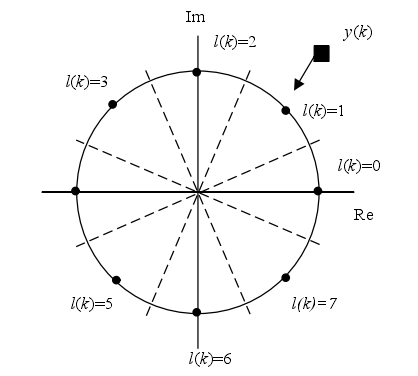
\includegraphics[width=0.5\textwidth]{figmutihopcomplex.png}
	\caption{复值神经元状态$(K=8)$及状态转移规则}
	% 图片标签,可用<\figref{}>引用
     \label{figmulti}
\end{figure}

其中激活函数$\csign(\cdot)$定义如下:
\begin{equation}
\csign(u)=
\left\{
\begin{array}{cc}
	e^{i0},&0\ls\arg[u\cdot\exp(i\pi/K)]<\frac{2\pi}{K}\\
	e^{i\frac{2\pi}{K}},&\frac{2\pi}{K}\ls\arg[u\cdot\exp(i\pi/K)]<\frac{4\pi}{K}\\
	\vdots&\vdots\\
	e^{i\frac{2\pi}{K}(K-1)},&(K-1)\frac{2\pi}{K}
	                                  \ls\arg[u\cdot\exp(i\pi/K)]<2\pi\\
\end{array}
\right.
\end{equation}

可见,激活函数$\csign(\cdot)$实际上可理解为一种复数域上定义的signum函数,它将神经元状态的加权和映射到了复平面单位圆上最接近该加权和的量化点上,其间加权和幅值固定映射成了1。相应的状态转移过程如\figref{figmulti}所示。

从激活函数的定义还可以看出,这种网络是一种全连接回归,且由于神经元的状态有$K$种$(K\gs2)$,因此可将该网络看作传统的二值Hopf\/ield神经网络在复数多值域中的扩展。于是,沿袭Hopf\/ield网络的状态更新方式,该类网络的状态更新也可分同步和异步两种:

异步方式:网络中的神经元状态等概率地依\equref{eqiter}进行更新,一次只更新一个神经元状态;

同步方式:网络的每次迭代中,所有神经元状态同时被更新,即依照下式更新:\begin{equation}
{\mathbf{ X}}(k+1)=\mathbf{ Y}(k)=\csign[\mathbf{ W }\cdot\mathbf{ X }(k)]               
\end{equation}
其中$\mathbf{ X}(k)$为神经元状态$x(k)$组成的列向量,$\mathbf{ W}=(w_{kj})$为整个网络的连接权矩阵。

% 节标题
\section{基于轻量级卷积神经网络的机器人智能抓取}

% 条标题
\subsection{机器人抓取检测的问题描述}

目前基于神经网络的机器人抓取位姿预测方法的研究主要集中在结合基础分类网络如 AlexNet、ResNet 等提高抓取检测准确性上,这些网络最初是为复杂的分类任务和海量数据的特点而设计的,网络结构通常具有大量的参数,需要大量的计算和存储资源。针对上述深度学习抓取检测方法的不足,文献\cite{bib:one}提出了基于 SqueezeNet 的轻量级卷积神经网络抓取预测模型,在不降低准确率的情况下,该网络模型更小,需要的存储资源更少,速度更快,更适合于移动机器人平台中。 类似的设计轻量级模型的工作如\cite{bib11}。

如\figref{figless1}所示的抓取位姿预测问题与如\figref{figless2}所示普通检测问题的区别在于:抓取位姿预测问题不只是在最佳抓取位置处预测出类似于普通检测问题形式的回归框,还要预测出最佳抓取位姿$(x,\ y,\ h,\ w,\ \theta)$。

\begin{figure}[!htbp]
	\centering
	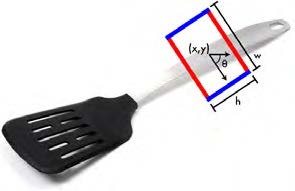
\includegraphics[width=0.4\textwidth]{less1.jpg}
	\caption{五维抓取表示}
     \label{figless1}
\end{figure}
\begin{figure}[!htbp]
	\centering
	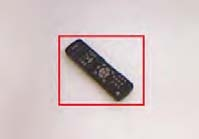
\includegraphics[width=0.3\textwidth]{less2.jpg}
	\caption{普通检测表示}
     \label{figless2}
\end{figure}

机器人抓取位姿检测问题可以被表述为对于给定对象的图像$I$找到最佳抓取位姿$g$。\figref{figless1}显示了一个五维抓取表示\upcite{bib3},以便对物体的潜在的最佳抓取位姿进行表示,五维抓取位姿$g$可以表示为\equref{eqgrasp}:
\begin{equation}
g=f(x,y,h,w,\theta)
\label{eqgrasp}
\end{equation}

其中$(x,\ y)$是与抓取矩形的中心对应的坐标,$h$是平行板的高度,$w$是平行板之间的最大距离,$\theta$是抓取矩形相对于水平轴的取向。蓝线$h$表示二指机器人手爪的平行板,红线$w$对应于抓取之前手爪的平行板之间的距离,该五维抓取表示给出了在对物体执行抓取时平行板夹具的位置和方向。Lenz 等表明一个最佳的五维抓取表示可以被映射回一个可以被机器人用来执行抓取的七维抓取表示,还可以降低计算成本。

% 条标题
\subsection{多模态轻量级抓取检测模型架构}

与以前的方法\upcite{bib3,bib4,bib5}相比,文献\cite{bib:one}使用一个小型轻量级的卷积神经网络架构 SqueezeNet-RM(SqueezeNet Regression Model),该架构结合 SqueezeNet\upcite{bib12}参数少的优点和 DenseNet\upcite{bib13}多旁路连接加强特征复用的思想能提升抓取检测准确率的优点,在康奈尔抓取数据集检测任务上,在保证准确率不降低的情况下,网络模型更小,所需存储空间更少,模型速度更快。

如\figref{figflowchart}所示,整体架构的思想是在 SqueezeNet 网络模型中引入 DenseNet 增加旁路加强特征复用的思想,conv1 和 conv10 之后加入 Batch Normalization,并在最后一层后面添加一个全连接层。全连接层有六个输出神经元对应抓取矩形框的坐标,四个神经元对应位置和高度,抓取角度使用两个附加的参数化坐标:正弦和余弦的两倍角。网络直接从原始图像回归出抓取位姿$(x,y,h,w,\theta)$。

\begin{figure}[!htbp]
	\centering
	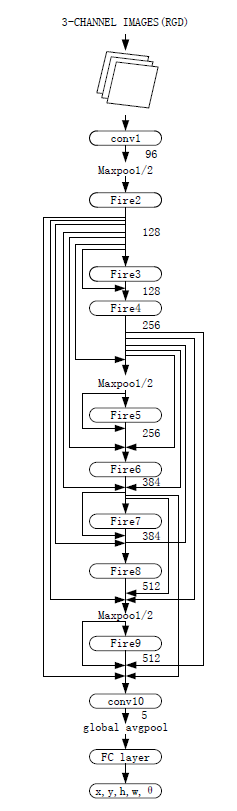
\includegraphics[width=0.4\textwidth]{flowchart}
	\caption{SqueezeNet-RM 网络模型}
     \label{figflowchart}
\end{figure}

% 条标题
\subsection{SqueezeNet轻量级卷积神经网络架构}

如\figref{figflowchart}, SqueezeNet-RM 网络模型以一个独立的卷积层 conv1 为开端,相邻的是 8 个 f\/ire 模块,之后加一个独立的卷积层 conv10,最后以一个最终的全连接层结束。在层 conv1,f\/ire4,f\/ire8 和 conv10 之后使用步长为 2 的 max-pooling、f\/ire2、f\/ire4、f\/ire6 分别向后面的每一层引出旁路连接,这些相对较后的 pooling 和旁路连接有助于提高检测精度。 

类似于 Inception\upcite{bib14}和 DenseNet\upcite{bib15}的模块化思想,SqueezeNet 神经网络采用了模块化的设计思想,它的基础模块称为 f\/ire 模块,如\figref{figfire}所示:  f\/ire 模块含两部分:squeeze 层和 expand 层。首先使用$1\times1$的卷积操作对输入特征图进行压缩,其卷积核数要少于上一层 feature map 数,输出特征图的数量可以远比输入特征图的数量少,这是 squeeze层的设计。然后,采用不同大小的卷积核$1\times1$和$3\times3$进行卷积操作,将这些卷积操作的输出特征图 concat 起来,这是 expand 层操作,最终将特征图的数量提升上去。将上述 f\/ire 模块堆叠, 得到 SqueezeNet 网络。

\begin{figure}[!htbp]
	\centering
	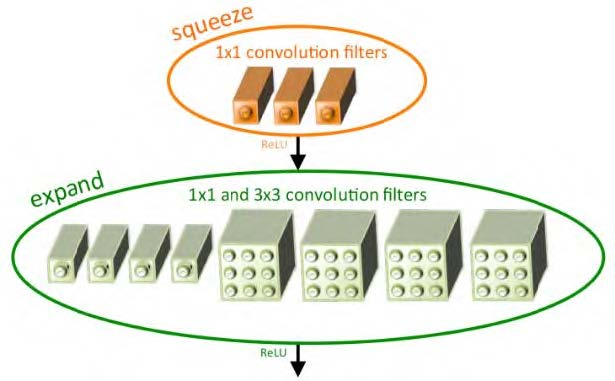
\includegraphics[width=0.6\textwidth]{less3}
	\caption{f\/ire模块}
     \label{figfire}
\end{figure}

SqueezeNet 通过 f\/ire 模块和自身优化结构,采用了以下几种常用的策略实现参数的减少。策略 1: 使用$1\times1$过滤器替换$3\times3$过滤器,因为$1\times1$滤波器具有比$3\times3$滤波器少9倍的参数,见\figref{figfire}中 Squeeze 层。策略 2:使用 Squeeze 层将输入到$3\times3$过滤器的通道的数量减少。具体而言,对于一个完全由$3\times3$滤波器组成的卷积层,该层中的参数的总量是(输入通道的数量)$\times$(滤波器的数量)$\times3\times3$,因此,为了在 CNN 中保持小的参数总数,在采用策略1的同时还要减少$3\times3$滤波器的输入通道的数量。策略 3:延迟降采样, 以使卷积层具有大的激活图,见\figref{figflowchart}中的 Maxpool 位置,大的激活图(通过延迟降采样)可以获得更高的检测精度,有助于提高任务的准确性\upcite{bib16}。策略1和2在试图保持准确性的同时减少CNN中的参数的数量,策略3是在有限的参数运算量上最大化精度。 

文献\cite{bib:one}采用在ImageNet分类问题上表现最佳的SqueezeNet (Simple Bypass  Conection) 架构\upcite{bib12}。 SqueezeNet是一个全卷积网络,在f\/ire9 层之后添加了一个随机失活层dropout\upcite{bib17},以避免过拟合,在 SqueezeNet 网络的最后一层添加一个全连接层Fully Connected Layer (FC层) 作为输出层。

% 节标题
\section{基于级联卷积神经网络的机器人智能抓取}

% 条标题
\subsection{机器人抓取检测的问题}

机器人抓取检测问题包括 2 个部分:抓取位置确定和抓取姿态估计。传统的位置检测方法根据二值化的图像计算物体重心作为抓取位置,但是可抓取位置不在重心处的物体甚多。通常采用滑动窗口法\upcite{bibb6,bibb7} 解决抓取点不在重心上的问题,但此方法以遍历搜索获得最优解,时间代价大。文\cite{bibb8} 对此作出了改进,通过缩小搜索区域范围并减少搜索窗旋转次数来实现时间的优化。Pinto 等人\upcite{bibb9}尝试用随机采样法缩短定位时间,但检测结果因依赖采样位置而表现不稳定,且计算时间减少的成效不明显。 在抓取姿态估计方面,文\cite{bibb7,bibb10}将最优搜索窗的旋转角度作为抓取角度,文\cite{bibb9} 率先以旋转角度为标签将抓取检测感知部分当作分类问题解决,但这些属于粗估计方法,低精度的抓取角度可导致机器人在实际抓取时因受力点错误而抓取失败。因此,减少抓取定位时间消耗和提升姿态估计精度是机器人在线抓取检测时亟待解决的 2 个问题。

深度神经网络用于机器人抓取位姿检测的另一个问题是,已有公开模型如文\cite{bibb7}和文\cite{bibb11}所提出的模型等都是在封闭大数据集上训练所得,通常需要随机器人部署而扩展关于实际特定抓取对象的小样本数据集。迁移学习为特定任务小样本集下深度网络模型训练提供了方法。自建的数据集规模虽小,但能够在已经过百万级封闭数据集训练并具有基本特征提取能力的模型上微调训练,令在特定小样本集下训练的模型仍具有卓越的性能。这样不仅能缩短训练周期,还可提升整个系统的拓展性。

文献\cite{bib:three}针对任意姿态的未知不规则物体,提出一种适于顶抓策略的平面抓取位姿快速检测方法,其主要研究内容及贡献包括:

% enumerate,有序列表环境
% fullwidth,正文不缩进
% label,设置编号格式,可选:\Alph \alph \Roman \roman 或 \arabic
% itemindent,编号缩进量
\begin{enumerate}[fullwidth, label=(\arabic*), itemindent=2em]
\item 提出一种抓取姿态细估计的卷积神经网络模型 Anlge-Net。

\item 在此基础上,提出一种两阶段级联式抓取位姿检测模型。模型第 1 阶段先以基于区域的全卷积网络\upcite{bibb12}为基础提取少量且可靠的候选抓取位置, 再对候选结果筛选排序确定最优抓取位置,以此加快检测速度;第 2 阶段为 Angle-Net 在前一阶段输出的局部位置图像下计算抓取角度。 相比于文\cite{bibb9}的方法,直接计算的抓取角度误差更小,抓取检测精度得以提升。
\end{enumerate}

% 条标题
\subsection{机器人抓取问题描述}

机器人平面抓取作业任务如\figref{figgrasp}所示。机器人视觉系统分析给定抓取场景的彩色图像,推断出顶抓策略下的目标物体最优抓取位姿。

\begin{figure}[!htbp]
	\centering
	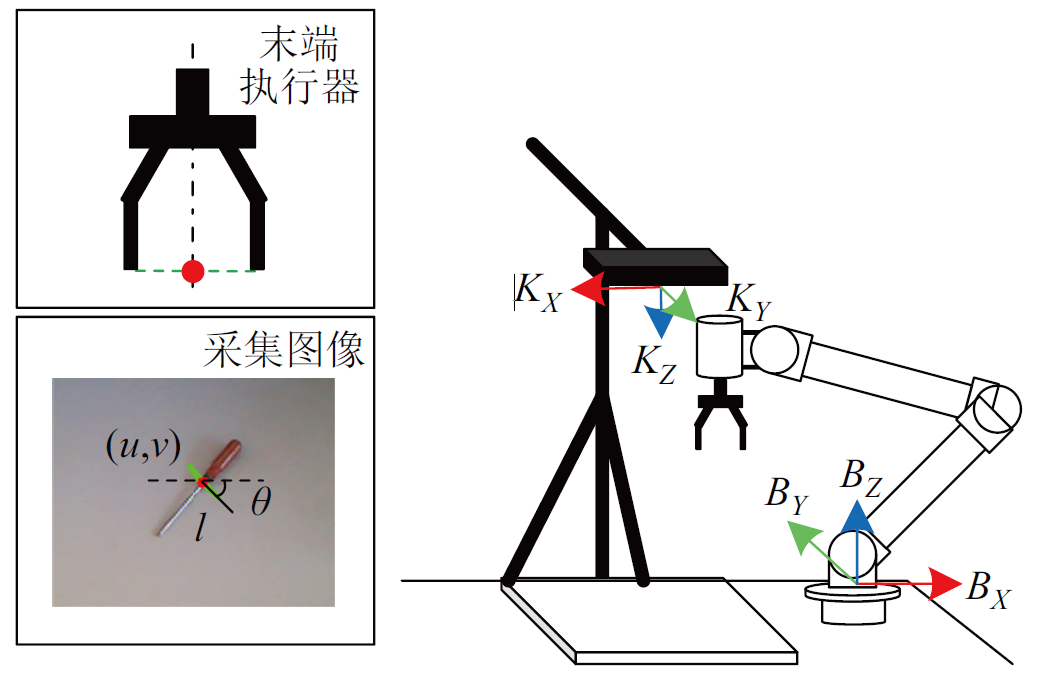
\includegraphics[width=0.6\textwidth]{3grasp}
	\caption{机器人抓取作业任务示例}
     \label{figgrasp}
\end{figure}

为使抓取检测结果与机器人末端执行器位姿对应,图像中抓取位姿检测结果采用基于文\cite{bibb4}方法简化得到的“点线法”表示,如\figref{figgrasp}中的采集图像部分所示,圆点为抓取位置的中心点,图像坐标系下记作$(u, v)$,对应机器人末端执行器两指连线的中点;短实线对应机器人末端执行器的两指连线,抓取角度$\theta$为该线顺时针旋转时与图像坐标系下$X$轴正方向的夹角,对应机器人末端执行器绕机器人 基坐标系$Z$轴旋转的角度。考虑到抓取角度的对称性,设$\theta\in [0, 180)$。线长$l$对应机器人末端执行器尝试抓取时的两指开度。

针对上述研究目标和相关定义,机器人抓取检测问题可描述如下:$t$时刻机器人获取目标的$n$维度特征序列$X (t) = (x_1(t), x_2(t),\cdots, x_n(t))$,有
\begin{equation}
G(u(t), v(t), \theta(t), l(t)) = F(X (t))
\end{equation}

其中,$F$为级联机器人平面抓取位姿检测模型,$G$为“点线法”表示的抓取检测结果。

% 条标题
\subsection{R-FCN与Angle-Net级联的抓取检测器}

抓取位姿检测任务包括抓取点确定和抓取姿态估计 2 个阶段。采取由粗到细的方式,针对各部分任务设计对应的卷积神经网络,并将网络级联成最终的检测模型。

模型结构如\figref{figpoe}所示,第 1 个阶段可视作定位与分类问题,以 R-FCN 为基础实现抓取定位以及抓取角度的粗估计;第 2 个阶段转换成回归问题,通过构造 Angle-Net 模型实现抓取角度的精细估计。

\begin{figure}[!htbp]
	\centering
	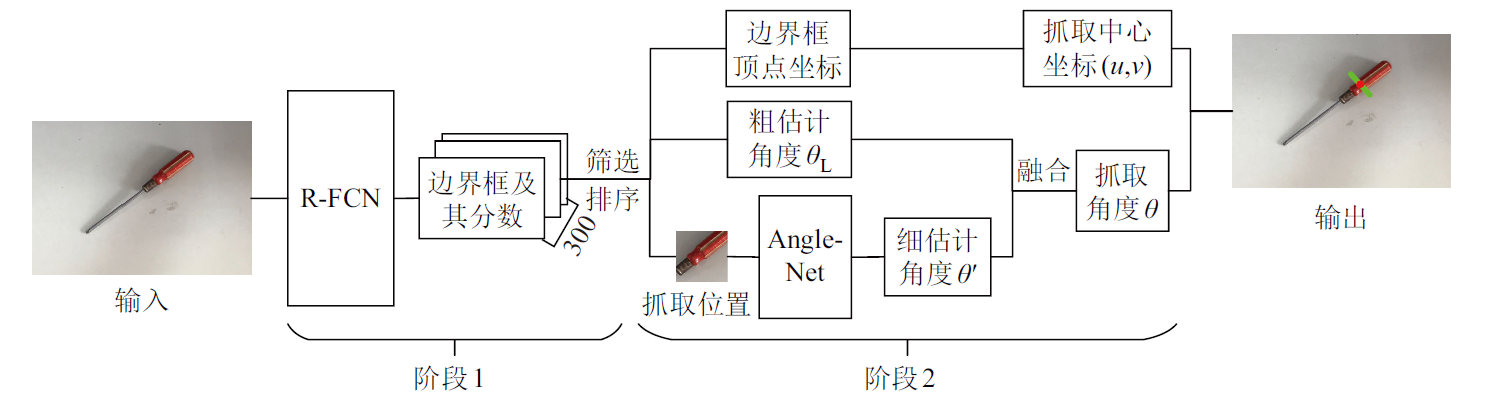
\includegraphics[width=\textwidth]{3posoreest}
	\caption{抓取位姿检测模型结构}
     \label{figpoe}
\end{figure}

针对目标检测问题已提出了许多优秀的深度学习模型,根据文\upcite{bibb14}的研究,基于区域的全卷积网络(R-FCN)兼具优秀的检测速度和准确率。故本文选用 R-FCN 实现图像中候选抓取位置的提取, 可抓取位置在图像上由边界框(bounding-box)标出,抓取点即为边界框中心点.为实现抓取角度的 粗估计,以抓取角度$\theta$为分类标签,共计 4 类:$0\degree,\ 45\degree,\ 90\degree,\ 135\degree$。为在提高检测速度的同时尽量降低对检测结果的影响,抓取位置候选框定为 300 个。 R-FCN 模型输入为任意尺寸的包含目标物体的场景图像,输出为候选框及其对应的可靠性分数,通过筛选和排序确定在工作区域内分数最高的抓取位置。

深度网络目标检测模型根据感兴趣区域(RoI)池化层分为两大类:一类是共享计算的全卷积子网络模型,如 R-CNN\upcite{bibb15}、 快速 R-CNN\upcite{bibb16}、 更快 R-CNN \upcite{bibb17};另一类为不共享计算的作用于各自 RoI 的子网络模型,如 SSD (single shot multibox detector)\upcite{bibb18}、YOLO (you only look once) \upcite{bibb19}。R-FCN 基于 R-CNN 的框架,即先进行区域建议再进行区域分类的策略,为了使检测能对目标的平移做出准确 响应,采用全卷积网络(FCN),用专门的卷积层构建位置敏感分数图 (position-sensitive score map)。每个空间敏感地图对 RoI 的相对空间位置信息进行编码,并在 FCN 上面增加 1 个位置敏感的RoI池化层来监管这些分数图。R-FCN 的结构如\figref{figrfcn}所示。

\begin{figure}[!htbp]
	\centering
	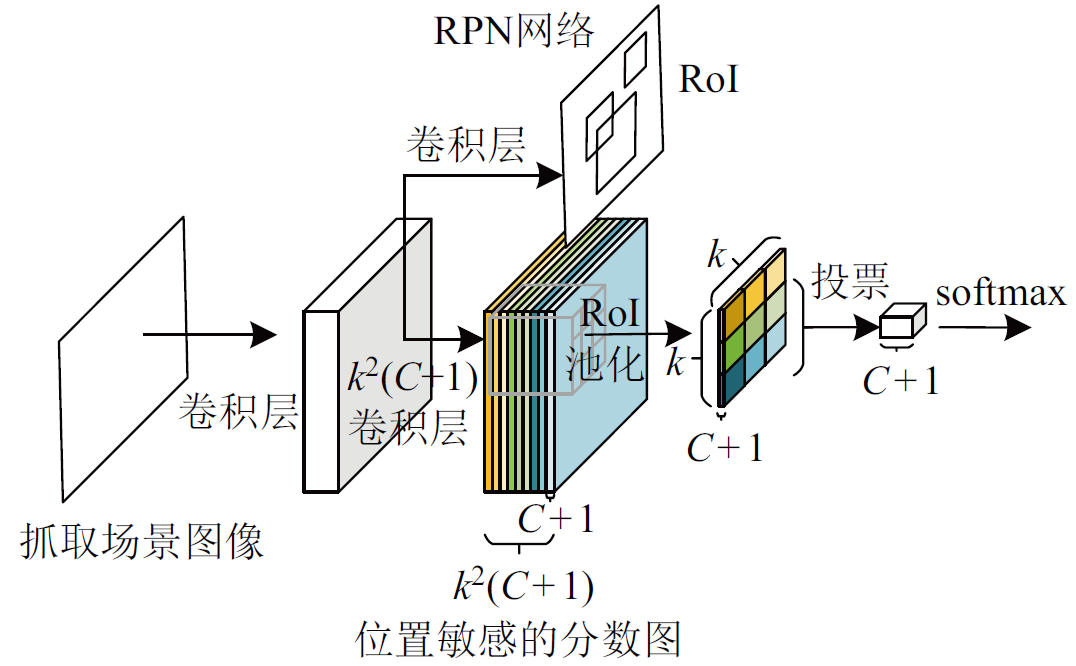
\includegraphics[width=0.6\textwidth]{3rfcn}
	\caption{R-FCN 模型结构}
     \label{figrfcn}
\end{figure}

设待检测类别共有$c$类,在机器人抓取检测模型中$c = 4$。R-FCN 结构中的基础卷积网络基于残差网络(ResNet)\upcite{bibb20},采用 ResNet 的前 100 层并在其最后接一个$1\times1\times1024$的全卷积层。基础卷积网络用于特征提取并输出特征图。区域建议网络沿用更快R-CNN中的区域建议网络(region proposal network,RPN)\upcite{bibb17}网络,生成多个 RoI,即抓取位置候选区域,每个 RoI 被分成$k\times k$块。$k^2$位置敏感分数图作为 R-FCN 中的最后一层卷积层,其功能是输出用于分类的结果。R-FCN 中对RoI 的$(i, j)$块$(0\ls i, j\ls k-1)$进行位置敏感的池化操作,定义为\equref{eqrcijt}:
\begin{equation}
r_c(i,j\mid\theta)=\sum_{(x,y)\in(i,j)}\frac{z_{i,j,c}(x+x_0,\ y+y_0|\Theta)}{n}
\label{eqrcijt}
\end{equation}

其中,$r_c(i,j\mid\theta)$表示$ (i, j) $块对第$ C $类的池化响应;$z_{i,j,c}$是 $k^2(4 + 1)$分数图中的一个,$(x_0, y_0)$ 表示 RoI 的左上角;$n$表示的是每一块当中的像素值,$\Theta$为待学习参数。

池化操作后输出$k^2$个位置敏感的分数图,利用\equref{eqrc}和\equref{eqsc}得到每一类最终的分数,用于计算损失。
\begin{equation}
r_c(\Theta)=\sum_{i,j}r_c(i,j\mid\theta)
\label{eqrc}
\end{equation}
\begin{equation}
s_c(\Theta)=\dfrac{\exp[{r_c(\Theta)}]}{\sum\limits_{c'=0}^C\exp[{r_{c'}(\Theta)}]}
\label{eqsc}
\end{equation}

用模型直接输出角度值替代角度分类标签值可实现更高精度的抓取姿态估计,故构建姿态细估计模型 Angle-Net,结构如\figref{figangle}所示。

\begin{figure}[!htbp]
	\centering
	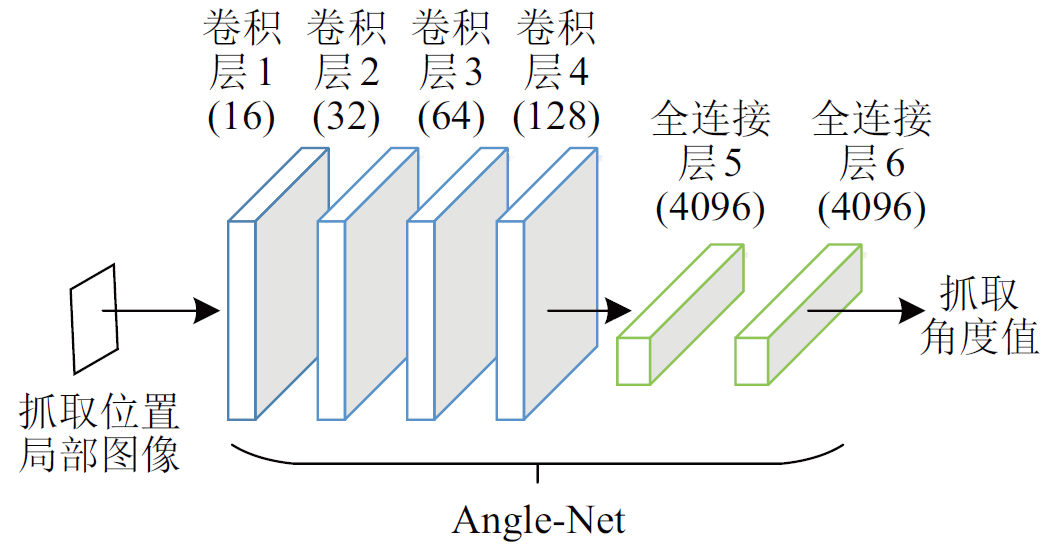
\includegraphics[width=0.6\textwidth]{3angle}
	\caption{Angle-Net 结构}
     \label{figangle}
\end{figure}

Angle-Net 由 4 个卷积层和 2 个全连接层组成。卷积层的卷积核个数分别为 16、 32、 64、 128,全连接层的神经元个数均为 4096。 损失函数(loss function)作为模型预测值与真实值差异程度的估量函数,决定了模型训练的收敛速度和最终效果。 Angle-Net 的损失函数采用L1范数函数,为防止过拟合,在损失函数的基础上加上正则化项,定义如\equref{eqnor}:
\begin{equation}
L=\frac{1}{N}\left(\Big|\theta'-\theta_0\Big|+\sum\limits_i^n\lambda\omega_i^2\right)
\label{eqnor}
\end{equation}
其中,$\theta_0$为期望的抓取角度,$\lambda$为正则化项,$\omega_i$为模型权值参数。

\subsubsection{四级标题示例}

% 条标题
\section{表格绘制示例}

表格按规定为五号字,引用表格示例:\tabref{symbol}.

% 第一列不用填写,自动编号的三线表
% 设置表格第一列计数器归零
\setcounter{rowno}{0}
\begin{center}
\renewcommand{\arraystretch}{1.25}
\begin{table}[H]
\centering %居中
\setlength{\abovecaptionskip}{0pt}
\setlength{\belowcaptionskip}{0pt}
\caption{符号说明}\label{symbol}
\begin{tabular}{>{\stepcounter{rowno}\therowno}ccl}
 \toprule[1.5pt]
\multicolumn{1}{c}{序号}& \makebox[0.2\textwidth][c]{符号}	&  \makebox[0.4\textwidth][c]{意义} \\ \midrule
 &$CNCi\#$&编号为$i$的CNC, $i=1,2,\cdots,8$\\
 &$t_{mj}$    & RGV移动$j$个单位所需时间, $j=0,1,2,3$ \\ 
 &$t_{cnc}$    & CNC加工完成一道工序的物料所需时间 \\ 
 &$t_{cnc1}$    & CNC加工完成第一道工序所需时间 \\ 
 &$t_{cnc2}$    & CNC加工完成第二道工序所需时间 \\ 
\bottomrule[1.5pt]
\end{tabular}
\end{table}
\end{center}

定义定理等环境示例:模板支持以下环境:definition、theorem、proposition、corollary、lemma、remark、exam、exer、note、proof、assumption、conclusion、solution,第二对\{\}内的内容为此定理的label,可以用此label引用,定理\ref{thm:sin}如下。
\begin{theorem}{正弦定理}{thm:sin}
\begin{equation}
\frac{a}{\sin A}=\frac{b}{\sin B}=\frac{c}{\sin C}
\end{equation}
\vspace{0.01cm}
\end{theorem}
% 证明环境
\begin{proof}
以下是一段无意义文字:\lipsum[5]
\end{proof}

如果需要对公式的子公式进行编号,则使用\lstinline{subeqnarray}环境:
\begin{lstlisting}
\begin{subeqnarray}
\label{eqw}
\slabel{eq0}
x & = & a \times b \\
\slabel{eq1}
& = & z + t\\
\slabel{eq2}
& = & z + t
\end{subeqnarray}
\end{lstlisting}
上述代码输出如下:
\begin{subeqnarray}
\label{eqw}
\slabel{eq0}
x & = & a \times b \\
\slabel{eq1}
& = & z + t\\
\slabel{eq2}
& = & z + t
\end{subeqnarray}

\equref{eqw}中,\lstinline{eqw}为整个公式的标签,\lstinline{slabel}为子公式的标签。

% 第4章
%% !TEX root = ../main.tex



% 第5章
%% !TEX root = ../main.tex

% 第6章
%% !TEX root = ../main.tex

% 结论
% !TEX root = ../main.tex

% 结论
\chapter*{结\quad 论}
\addcontentsline{toc}{chapter}{结\quad 论}

学位论文的结论作为论文正文的最后一章单独排写,但不加章标题序号。结论是对整个论文主要成果的总结。在结论中应明确指出本研究内容的创新性成果或创新点(含新见解、新观点),并指出今后进一步在本研究方向进行研究工作的展望与设想,上述各项用(1).(2).  $\cdots$表述,不要将结论写成论文的摘要。结论字数一般在2000字以内。

% 参考文献
% !TEX root = ../main.tex

% 参考文献
% 文献个数小于99
\begin{thebibliography}{99}
\addcontentsline{toc}{chapter}{参考文献}

% 每条参考文献均需用<\bibitem{}>引出,
% 花括号里的内容为此条参考文献的标签label,
% 可用<\upcite{}>和<\cite{}>引用。

\bibitem{bibc1} 焦李成.神经网络系统理论[M].西安:西安电子科技大学出版社,1991.
\bibitem{bibc2} 何玉彬,李新忠.神经网络控制及其应用[M].北京:科学出版社,2000.
\bibitem{bibc3} McCulloch W S, Pitts W A. A logical calculus of the ideas immanent in nervous activity[J]. Bulletin of Mathematical Biophysics, 1943, 5: 115-133.
\bibitem{bibc4} Hebb D O. The Organization of Behaviour [M]. New York, John Wiley\&Sons Inc., 1949.
\bibitem{bibc5} Rosenblatt. The perception: a probabilistic model for information storage and organization in the brain [J]. Psychology Review, 1958, 65: 386-408.
\bibitem{bibc6} Minsky M, Papert S. Perceptron [M]. Cambridge, MA: MIT Press, 1969.
\bibitem{bibc7} Hopf\/ield  J  J.  Neural  networks  and  physical  systems  with  emergent  collective computational  abilities[C].  Proceeding  of the National Academy  of  Science.  USA (Biophysics), 1982, 79: 2554-2558.
\bibitem{bibc8} Hopf\/ield J J. Neurons with graded response have collective computational properties like those  of  two-state  neurons[C].  Proceedins  of  the  National  Academy  of  Science, USA(Biophysics), 1984, 81:3088-3092.
\bibitem{bibc9} Widrow B, McCool J, Ball M. The complex LMS algorithm [C]. Proc. IEEE, 1975, 63(4):719-720
\bibitem{bibc10} Hirose  A.  Complex-valued  neural  networks:  theories  and  applications  [M].  World Scientif\/ic Series on Innovation Intelligence, vol 5, Singapore: World Scientif\/ic Publishing Co. Pte. Ltd. 2003

\bibitem{bib1} 谢林江, 季桂树, 彭清, 等. 改进的卷积神经网络在行人检测中的应用[J].  计算机科学与探索,  2018,  12(5):708-718.
\bibitem{bib2}王耀玮, 唐伦, 刘云龙, 等. 基于多任务卷积神经网络的车辆多属性识别[J].  计算机工程与应用, 2018, 54(8):21-27.
\bibitem{bib3} Lenz I, Lee H, Saxena A. Deep learning for detecting robotic grasps[J]. The International Journal of Robotics Research, 2015, 34(4-5):705-724.
\bibitem{bib4} Kumra S, Kanan C. Robotic grasp detection using deep convolutional neural networks[C]//2017 IEEE/RSJ International Conference on Intelligent Robots and Systems (IROS). IEEE, 2017: 769-776.
\bibitem{bib5} Chu F J, Xu R, Vela P A. Real-world multiobject, multigrasp detection[J]. IEEE Robotics and Automation Letters, 2018, 3(4): 3355-3362.
\bibitem{bib6}  Robot Learning Lab: Learning to Grasp[EB/OL].(2009) [2019-03-12].
\bibitem{bib7}  Redmon J, Angelova A. Real-time grasp detection using convolutional neural networks[C]//2015 IEEE International Conference on Robotics and Automation (ICRA). IEEE, 2015: 1316-1322.
\bibitem{bib8} Ni P, Zhang W, Bai W, et al. A New Approach Based on Two-stream CNNs for Novel Objects Grasping in Clutter[J]. Journal of Intelligent \& Robotic Systems, 2018(2):1-17.
\bibitem{bib9} Krizhevsky A, Sutskever I, Hinton G E. Imagenet classif\/ication with deep convolutional neural networks[C]// Advances in neural information processing systems. 2012: 1097-1105.
\bibitem{bib10} He K, Zhang X, Ren S, et al. Deep residual learning for image recognition[C]//Proceedings of the IEEE conference on computer vision and pattern recognition. 2016: 770-778.

\bibitem{bibb1} Dogar M, Hsiao K, Ciocarlie M, et al. Physics-based grasp planning through clutter[C]//Robotics: Science and Systems VIII. Cambridge, USA: MIT Press, 2012: 8pp.
\bibitem{bibb2} Goldfeder C, Ciocarlie M, Dang H, et al. The Columbia grasp database[C]//IEEE International Conference on Robotics and Automation. Piscataway, USA: IEEE, 2009: 1710-1716.
\bibitem{bibb3} Weisz J, Allen P K. Pose error robust grasping from contact wrench space metrics[C]//IEEE International Conference on Robotics and Automation. Piscataway, USA: IEEE, 2012: 557- 562.
\bibitem{bibb4}   Jiang Y, Moseson S, Saxena A. Eff\/icient grasping from RGB-D images: Learning using a new rectangle representation[C]// IEEE International Conference on Robotics and Automation. Piscataway, USA: IEEE,2011: 3304-3311.
\bibitem{bibb5}  Hinton G E, Salakhutdinov R R. Reducing the dimensionality of data with neural networks[J]. Science, 2006, 313(5786): 504-507.

\bibitem{bib11} Qiang Z, Li Z, Li J, et al. Vehicle color recognition using
Multiple-Layer Feature Representations of lightweight convolutional neural network[J]. Signal Processing, 2018, 147: 146-153. 

 \bibitem{bib:one} 马倩倩,李晓娟,施智平.轻量级卷积神经网络的机器人抓取检测研究[J/OL].计算机工程与应用:1-11[2019-04-09].
 
 \bibitem{bib12} Iandola F N, Han S, Moskewicz M W, et al. SqueezeNet: AlexNet-level accuracy with 50x fewer parameters and<
0.5 MB model size[J].2016.

 \bibitem{bib13} Huang G, Liu Z, Van Der Maaten L, et al. Densely connected convolutional networks[C]//Proceedings of the IEEE conference on computer vision and pattern recognition, 2017: 4700-4708.

 \bibitem{bib14} Szegedy C, Vanhoucke V, Ioffe S, et al. Rethinking the inception architecture for computer vision[C]// Proceedings of the IEEE conference on computer vision and pat- tern recognition. 2016: 2818-2826.
 \bibitem{bib15} Huang G, Liu Z, Van Der Maaten L, et al. Densely connected convolutional networks[C]//Proceedings of the IEEE conference on computer vision and pattern recognition. 2017: 4700-4708.
 \bibitem{bib16} He K, Sun J. Convolutional neural networks at con-strained time cost[C]//Proceedings of the IEEE conference on computer vision and pattern recognition. 2015: 5353-5360.
 \bibitem{bib17} Srivastava N, Hinton G, Krizhevsky A, et al. Dropout: a simple way to prevent neural networks from overfitting[J]. The Journal of Machine Learning Research, 2014, 15(1): 1929-1958.

\bibitem{bibb6}   仲训杲,徐敏,仲训昱,等.基于多模特征深度学习的机器人抓取判别方法 [J].自动化学报,2016,42(7):1022- 1029.
\bibitem{bibb7} Lenz I, Lee H, Saxena A. Deep learning for detecting robotic grasps[J]. International Journal of Robotics Research, 2015, 34(4/5): 705-724.
\bibitem{bibb8}   杜学丹,蔡莹皓,鲁涛,等.一种基于深度学习的机械臂抓取方法  [J].机器人,2017,39(6):820-828,837.
\bibitem{bibb9} Pinto L, Gupta A. Supersizing self-supervision: Learning to grasp from 50k tries and 700 robot hours[C]//IEEE International Conference on Robotics and Automation. Piscataway, USA: IEEE, 2016: 3406-3413.
\bibitem{bibb10} Guo D, Sun F C, Liu H P, et al. A hybrid deep architecture for robotic grasp detection[C]//IEEE International Conference on Robotics and Automation. Piscataway, USA: IEEE, 2017: 1609-1614.
\bibitem{bibb11} 刘义军.基于 FPGA 的线结构光视觉测量系统研究 [D]. 长 春:吉林大学,2017:23-49.

 \bibitem{bib:three} 夏晶,钱堃,马旭东,刘环.基于级联卷积神经网络的机器人平面抓取位姿快速检测[J].机器人,2018,40(06):794-802.
 
\bibitem{bibb12} 邹媛媛,赵明扬,张雷.基于量块的线结构光视觉传感器直接标定方法 [J]. 中国激光,2014,41(11):189-194.
\bibitem{bibb13} 卢津,孙惠斌,常智勇.新型正交消隐点的摄像机标定方法 [J]. 中国激光,2014,41(2):294-302.

\bibitem{bibb14} Huang J, Rathod V, Sun C, et al. Speed/accuracy trade-offs for modern convolutional object detectors[A/OL]. (2017-04-25) [2017-12-07].    
\bibitem{bibb15} Girshick R, Donahue J, Darrell T, et al. Rich feature hierarchies for accurate object detection and semantic segmentation[C]//IEEE Conference on Computer Vision and Pattern Recognition. Piscataway, USA: IEEE, 2014: 580-587.
\bibitem{bibb16} Girshick R. Fast R-CNN[C]//IEEE International Conference on Computer Vision. Piscataway, USA: IEEE, 2015: 1440-1448.
\bibitem{bibb17} Ren S Q, He K M, Girshick R, et al. Faster R-CNN: Towards real-time object detection with region proposal networks[M]// Advances in Neural Information Processing Systems 28. Cam- bridge, USA: MIT Press, 2015: 91-99.
\bibitem{bibb18} Liu W, Anguelov D, Erhan D, et al. SSD: Single shot multibox detector[C]//European Conference on Computer Vision. Cham, Switzerland: Springer, 2016: 21-37.
\bibitem{bibb19} Redmon J, Divvala S, Girshick R, et al. You only look once: Unified, real-time object detection[C]//IEEE Conference on Computer Vision and Pattern Recognition. Piscataway, USA:IEEE, 2016: 779-788.
\bibitem{bibb20} Szegedy C, Ioffe S, Vanhoucke V, et al. Inception-v4, Inception-ResNet and the impact of residual connections on learning [A/OL]. (2016-08-23) [2017-12-07].

\bibitem{bib:two} 李传浩. 基于卷积神经网络的机器人自动抓取规划研究[D].哈尔滨工业大学,2018.
 
 \bibitem{bib:four} 胡琳,晁飞.基于双神经网络结构的发展型机器人3D抓取[J].电脑知识与技术,2012,8(12):2859-2862.
\bibitem{bib:five} 刘晓玉. 复杂环境下基于神经网络的工件识别与机器人智能抓取[D].武汉科技大学,2009.
\bibitem{bib:six} 游辉胜. 基于模糊神经网络的单目视觉伺服机器人智能抓取[D].武汉科技大学,2008.
\end{thebibliography}

% 原创性声明
\declaration

% 开始写附录
\appendix

% 附录A
% !TEX root = ../main.tex

% 注意:由于模板的一些限制,附录部分章节需要手动编号
% 附录的章节均需要使用带星号的版本
\chapter*{附录A\hskip.5em 外文资料翻译}
\addcontentsline{toc}{chapter}{附录A\hskip.5em 外文资料翻译}
% 设置章节编号为1,即A
\setcounter{chapter}{1}
% 重置所有计数器
\setcounter{equation}{0}
\setcounter{figure}{0}
\setcounter{table}{0}

题目:基于驾驶员—车辆—道路交互的驾驶安全场

期刊:IEEE Transactions on Intelligent Transportation Systems, 2015, 16: 2203-2214.

摘要:车辆驾驶安全受许多因素的影响,包括驾驶员、车辆和道路环境,它们之间的相互作用非常复杂。现有的评估驾驶安全性的方法仅考虑有限的因素及其相互作用,基于运动学和动力学的车辆驾驶安全辅助系统难以适应日益复杂的交通环境。在本文中,我们提出了一个新的概念——驾驶安全场。驾驶安全场利用场论来表示由驾驶员、车辆、道路状况和其他交通因素引起的风险因素。本文构建了一个统一的驾驶安全场模型,包括以下三个部分:(1)势能场,由道路上的静止物体构成,例如停止的车辆;(2)动能场,由道路上的移动物体构成,例如车辆和行人;(3)行为场,由驾驶员的个人特征构成。

\section*{A.1\hskip.5em 求和算子}

\textbf{求和算子} 是用以表达多个数求和运算的一个缩略符号,它在统计学和计量经济学分析中扮演着重要作用。如果 $\{x_i: i=1, 2, \cdots, n\}$ 表示 $n$ 个数的一个序列,那么我们就把这 $n$ 个数的和写为\equref{eq:1}:
\begin{equation}
\label{eq:1}
\sum_{i=1}^n x_i \equiv x_1 + x_2 +\cdots + x_n
\end{equation}

引用图片示例:\figref{appen:angle}

\begin{figure}[!htbp]
	\centering
	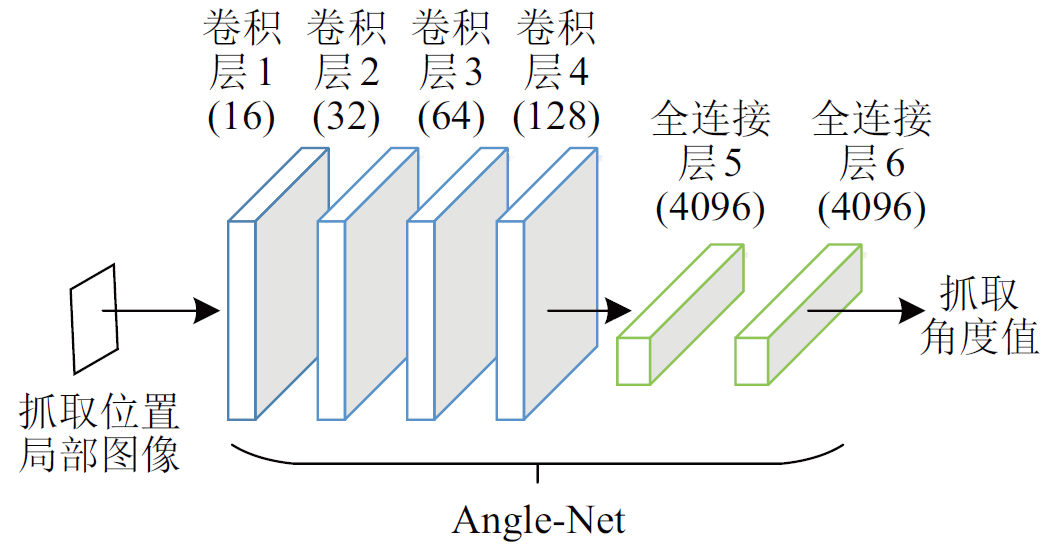
\includegraphics[width=0.6\textwidth]{3angle}
	\caption{附录插图示例:Angle-Net 结构}
     \label{appen:angle}
\end{figure}

% 附录B
% !TEX root = ../main.tex

\chapter*{附录B\hskip.5em 其他附录文本}
\addcontentsline{toc}{chapter}{附录B\hskip.5em 其他附录文本}
% 设置章节编号为1,即A
\setcounter{chapter}{2}
% 重置所有计数器
\setcounter{equation}{0}
\setcounter{figure}{0}
\setcounter{table}{0}

\lipsum[2]

\section*{B.1\hskip.5em 求和算子}

\textbf{求和算子} 是用以表达多个数求和运算的一个缩略符号,它在统计学和计量经济学分析中扮演着重要作用。如果 $\{x_i: i=1, 2, \cdots, n\}$ 表示 $n$ 个数的一个序列,那么我们就把这 $n$ 个数的和写为\equref{eq:2}:
\begin{equation}
\label{eq:2}
a^2+b^2=c^2
\end{equation}

引用图片示例:\figref{appen:fire}

\begin{figure}[!htbp]
	\centering
	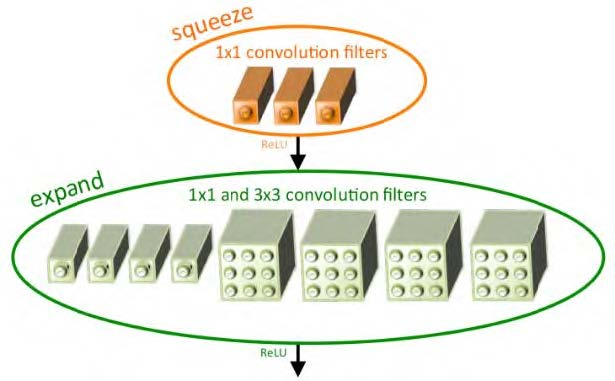
\includegraphics[width=0.6\textwidth]{less3}
	\caption{附录插图示例:f\/ire模块}
     \label{appen:fire}
\end{figure}

% 结束文档撰写
\end{document}
%%=============================================